% begin module volumes-otherline
\begin{frame}
\begin{example}[Rotation About a Line Parallel to the $x$-axis]
Find the volume of the solid obtained by rotating about the line $y = 1$ \alertNoH{4}{the region bounded by \alertNoH{2}{$y = -x^2+2x+1$} and \alertNoH{3}{$y = 1$}.}

\uncover<handout:2,3|13->{\alertNoH{13,14}{Cross-section:} \alertNoH{15,16}{a circle centered at \fcAnswerUncover{ 13}{16}{$(x, 1),$}}\\
\alertNoH{17,18}{radius: \fcAnswerUncover{ 13}{18}{$(-x^2 +2x + 1) -1, $}}\\ 
\alertNoH{19, 20}{area: $\alertNoH{24}{A(x)} =\fcAnswer{20}{ \pi \left((- x^2 + 2x + \fcCancel{21}{1})-\fcCancel{21}{1}  \right)^2} \uncover<21->{\alertNoH{24}{=\pi \left(-x^2+2x  \right)^2}.} $}
}%

\begin{columns}[c]
\column{0.35\textwidth}
\begin{pspicture}(-1,-2)(3,3)%
\tiny%
\fcBoundingBox{-1}{-0.7}{2.5}{2.5}%
\newcommand{\theFun}{u u mul -1 mul 2 u mul add 1 add\space}%
\newcommand{\theYAxis}{1\space}%
\newcommand{\theSurfaceFla}{u v cos \theFun \theYAxis sub mul \theYAxis add v sin \theFun \theYAxis sub mul\space}%
\newcommand{\theSurface}{%
\fcSurfaceInScene[colorVU= {0.7 0.2 0.2}, iterationsU=4, arrows=none, linewidth=0.3, linecolor=black ]{0.03}{0}{1.99}{30 \fcIterationsV\space mul}{[\theSurfaceFla]}{}%
}%
\renewcommand{\fcScreenStyle}{x}%
\renewcommand{\fcScreen}{[0 0 -1] 0}%
\renewcommand{\fcIterationsU}{4}%
\only<handout:2|5->{\renewcommand{\fcScreen}{[-0.03 -0.03 -1] 0}}%
\only<handout:2|6->{\renewcommand{\fcScreen}{[-0.06 -0.06 -1] 0}}%
\only<handout:2|7->{\renewcommand{\fcScreen}{[-0.12 -0.12 -1] 0}}%
\only<handout:2,3|8->{\renewcommand{\fcScreen}{[-0.15 -0.15 -1] 0}}%
\uncover<handout:1|4-12>{\pscustom*[linecolor=\fcColorAreaUnderGraph]{%
\fcLineIIId{ [0 1 0]}{[2 1 0]}%
\fcCurveIIId{2}{0}{[1 dict begin /u t def t \theFun 0 end]}%
}}%
\fcStartIIIdScene%
\fcAxesIIIdFullInScene[linewidth=1, linecolor=black, arrows=->, xLabel={$x$}, yLabel={$y$},zLabel={} ]{-0.5}{-0.5}{-3.2}{2.3}{2.3}{3.2}%
\only<handout:3|14-21>{%
\fcSurfaceInScene[colorUV=cyan, colorVU=cyan, linecolor=cyan, arrows=(none), iterationsV=22]{1.02 }{0 }{1 dict begin /u 0.5 def \theFun end }{ 360}{ [0.5 v cos u 1 sub  mul 1 add v sin u 1 sub mul] }{}%
}%
\only<handout:2|12,13,22->{%
\renewcommand{\fcIterationsV}{12}%
\theSurface%
}%
\only<handout:2,3|13,14-21>{\fcCurveIIIdInScene[linecolor=blue, linewidth=1]{0}{360}{2 dict begin /v t def /u 0.5 def [\theSurfaceFla] end}}%
\uncover<handout:2,3|5->{\fcPutIIId[t]{[0 0 3.1]}{$z$}}%
\only<handout:0|9>{%
\renewcommand{\fcIterationsV}{3}%
\theSurface%
\fcCurveIIIdInScene[arrows=(none), linecolor=red, linewidth=1.5]{0}{2}{[2 dict begin /v 90 def /u t def \theSurfaceFla end]}%
}%
\only<handout:0|10>{%
\renewcommand{\fcIterationsV}{6}%
\theSurface%
\fcCurveIIIdInScene[arrows=(none), linecolor=red, linewidth=1.5]{0}{2}{[2 dict begin /v 180 def /u t def \theSurfaceFla end]}%
}%
\only<handout:0|11>{%
\renewcommand{\fcIterationsV}{9}%
\theSurface%
\fcCurveIIIdInScene[arrows=(none), linecolor=red, linewidth=1.5]{0}{2}{[2 dict begin /v 270 def /u t def \theSurfaceFla end]}%
}%
\only<2->{\fcCurveIIIdInScene[arrows=(none), linecolor=red, linewidth=1.5]{0}{2}{[1 dict begin /u t def t \theFun 0 end]}}%
\only<3->{\fcLineIIIdInScene[linecolor=red, linewidth=1, arrows= (none)]{ [0 1 0]}{[2 1 0]}}%
\fcFinishIIIdScene%
\only<14-21>{\fcDotIIId{[0.5 1 0]}}%
\only<handout:1,3|16-21>{\fcPutIIId[lt]{[0.6 0.9 0]}{$(x,1)$}}%
\uncover<2->{\fcPutIIId[b]{[1.3 2.2 0]}{$y=-x^2+2x+1$}}%
\uncover<17-21>{\fcLineIIId[linecolor=red]{[0.5 1 0]}{[0.5 1 dict begin /u 0.5 def \theFun end  0]}}%
\uncover<23->{\fcLineIIId[linecolor=blue, linewidth=1.5pt]{[0 0 0]}{[2 0 0]}%
\uncover<23->{\fcPerpendicularIIId[linestyle=dashed]{[2 1 0]}{[1 0 0]}{0.1}}%
\fcDotIIId[linecolor=blue]{[0 0 0]}%
\fcDotIIId[linecolor=blue]{[2 0 0]}%
}%
\end{pspicture}
%\only<handout:0| 1>{%
%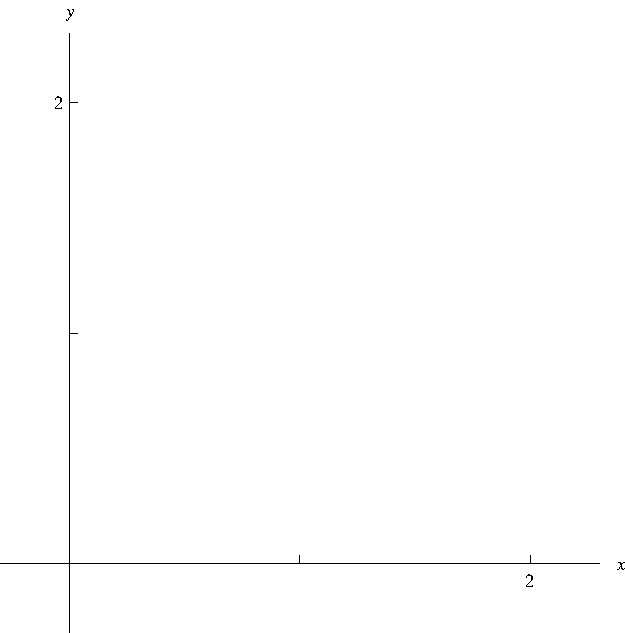
\includegraphics[height=2cm]{volumes/pictures/06-02-otherlinea.pdf} %
%}%
%\only<handout:0| 2>{%
%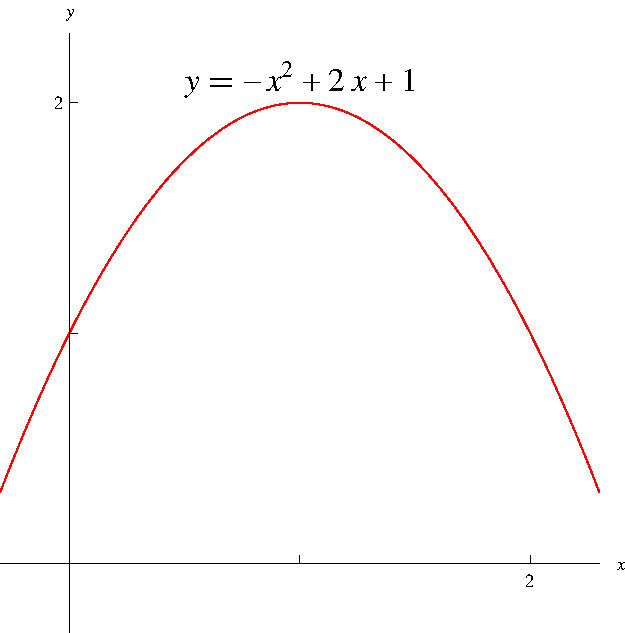
\includegraphics[height=2cm]{volumes/pictures/06-02-otherlineb.pdf} %
%}%
%\only<handout:0| 3>{%
%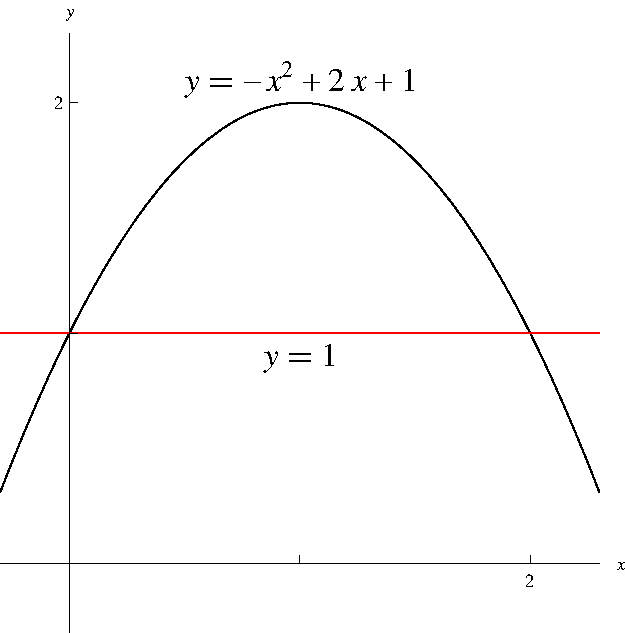
\includegraphics[height=2cm]{volumes/pictures/06-02-otherlinec.pdf} %
%}%
%\only<handout:0| 4>{%
%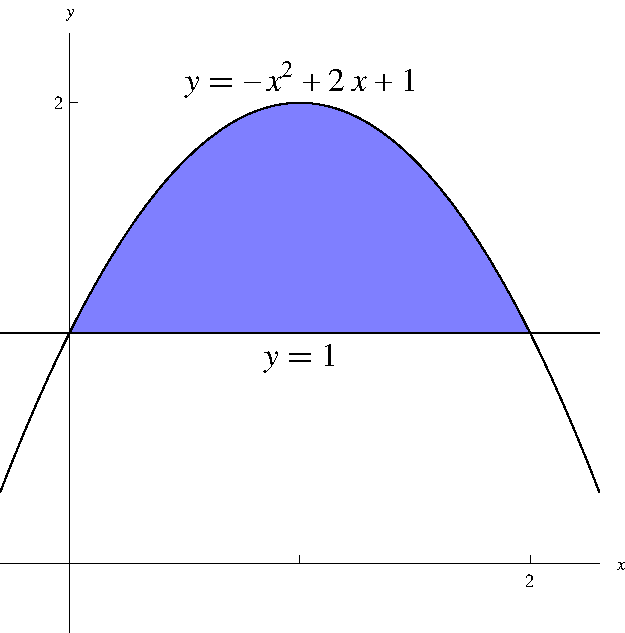
\includegraphics[height=2cm]{volumes/pictures/06-02-otherlined.pdf} %
%}%
%\only<5->{%
%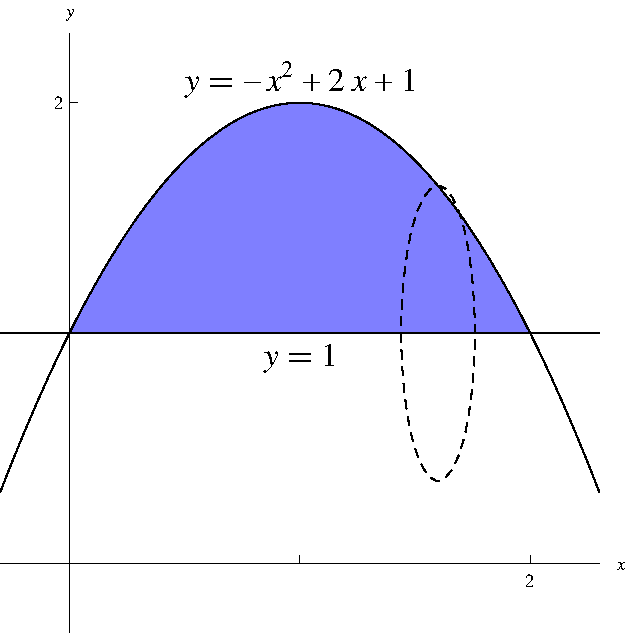
\includegraphics[height=2cm]{volumes/pictures/06-02-otherlinee.pdf} %
%}%
\column{0.65\textwidth}

\uncover<handout:3|1->{
$
\begin{array}{@{}r@{~}c@{~}l}
\uncover<22->{V&  = &\displaystyle \int_{{\fcAnswer{23}{ 0} }}^{{\fcAnswer{23}{2}} } \alertNoH{24}{A(x)} \diff x \uncover<24->{= \int_0^2 \alertNoH{24}{ \alertNoH{25}{\pi} \alertNoH{26}{\left( -x^2+2x\right)^2}  } \diff x%
}}\\%
\uncover<25->{&  = &\displaystyle \alertNoH{25}{\pi} {\alertNoH{27-32}{\int} }_{\!\!\!0}^2 \left(\alertNoH{26}{ \alertNoH{27,28}{x^4} - \alertNoH{29, 30}{4x^3} + \alertNoH{31,32}{4x^2}} \right)  \alertNoH{27-32}{\diff x} }\\%
\uncover<27->{&  =& \displaystyle \pi {\left[ \fcAnswerUncover{27}{28}{ \frac{ {\alertNoH{33,34}{x}}^5 }{5}} - \fcAnswerUncover{27}{30}{{\alertNoH{33,34}{x}}^4} + \fcAnswerUncover{27}{32}{ \frac{4 {\alertNoH{33,34}{x}}^3}{3}} \right] }_{ \alertNoH{34}{0}}^{\alertNoH{33}{2}}%
}\\%
\uncover<33->{&  = &\displaystyle  \pi \left( \frac{{\alertNoH{33}{2}}^5}{5} - {\alertNoH{33}{2}}^4 + 4\cdot\frac{{\alertNoH{33}{2}}^3}{3} \right)} \\
\uncover<35->{&=&\displaystyle \pi \left( \frac{32}{5} - 16 + \frac{32}{3} \right) = \frac{16}{15}\pi .}
\end{array}
$
}
\end{columns}
\end{example}
\end{frame}
% end module volumes-otherline
